%%%%%%%%%%%%%%%%%%%%%%%%%%%%%%%%%%%%%%%%%%%%%%%%%%%%%%%%%%%%%%%
%%%  notes
%%%%%%%%%%%%%%%%%%%%%%%%%%%%%%%%%%%%%%%%%%%%%%%%%%%%%%%%%%%%%%%

\documentclass[onecolumn,fleqn,notitlepage,secnumarabic]{revtex4}

% special 
\usepackage{ifthen}
\usepackage{ifpdf}
\usepackage{float}
\usepackage{color}

% fonts
\usepackage{latexsym}
\usepackage{amsmath} 
\usepackage{amssymb} 
\usepackage{bm}
\usepackage{wasysym}


\ifpdf
\usepackage{graphicx}
\usepackage{epstopdf}
\else
\usepackage{graphicx}
\usepackage{epsfig}
\fi

% packages added by jarondl
%
%\usepackage{subfig}  %% causes odd captions
\usepackage{verbatim} % for multiline comments
\usepackage{natbib} % change the bibliography style 
\usepackage{fancybox} % allows putting boxes with borders
\usepackage{cmap}  % for making pdf mathmode searchable
%\usepackage{sectsty}
\usepackage[pdftitle={Notes by Jarondl}]{hyperref}  % for hyperlinks in biblio. should be called last?

\graphicspath{{figures/},{PROG/figures/}}


%%%%%%%%%%%%%%%%%%%%%%%%%%%%%%%%%%%%%%%%%%%%%%%%%%%%%%%%%%%%%%%%


% NEW 
\newcommand{\abs}[1]{\left|#1\right|}
\newcommand{\Prob}{\mbox{Prob}\,}
\newcommand{\erf}{\mbox{erf}\,}
\newcommand{\barline}[1]{#1}

% math symbols I
\newcommand{\sinc}{\mbox{sinc}}
\newcommand{\const}{\mbox{const}}
\newcommand{\trc}{\mbox{trace}}
\newcommand{\intt}{\int\!\!\!\!\int }
\newcommand{\ointt}{\int\!\!\!\!\int\!\!\!\!\!\circ\ }
\newcommand{\ar}{\mathsf r}
\newcommand{\im}{\mbox{Im}}
\newcommand{\re}{\mbox{Re}}

% math symbols II
\newcommand{\eexp}{\mbox{e}^}
\newcommand{\bra}{\left\langle}
\newcommand{\ket}{\right\rangle}

% Mass symbol
\newcommand{\mass}{\mathsf{m}} 
\newcommand{\Mass}{\mathsf{M}} 

% more math commands
\newcommand{\tbox}[1]{\mbox{\tiny #1}}
\newcommand{\bmsf}[1]{\bm{\mathsf{#1}}} 
%\newcommand{\amatrix}[1]{\matrix{#1}} 
\newcommand{\amatrix}[1]{\begin{matrix} #1 \end{matrix}} 
\newcommand{\pd}[2]{\frac{\partial #1}{\partial #2}}

% equations
\newcommand{\mylabel}[1]{\label{#1}} 
%\newcommand{\mylabel}[1]{\textcolor{blue}{[#1]}\label{#1}} 
\newcommand{\beq}{\begin{eqnarray}}
\newcommand{\eeq}{\end{eqnarray}} 
\newcommand{\be}[1]{\begin{eqnarray}\ifthenelse{#1=-1}{\nonumber}{\ifthenelse{#1=0}{}{\mylabel{e#1}}}}
\newcommand{\ee}{\end{eqnarray}} 

% arrangement
\newcommand{\drawline}{\begin{picture}(500,1)\line(1,0){500}\end{picture}}
\newcommand{\bitem}{$\bullet$ \ \ \ }
\newcommand{\Cn}[1]{\begin{center} #1 \end{center}}
\newcommand{\mpg}[2][1.0\hsize]{\begin{minipage}[b]{#1}{#2}\end{minipage}}
\newcommand{\mpgt}[2][1.0\hsize]{\begin{minipage}[t]{#1}{#2}\end{minipage}}
\newcommand{\putgraph}[2][width=0.30\hsize]{\includegraphics[#1]{#2}}

% more
%\newcommand{\Eq}[1]{Eq.\!\!~(\ref{#1})}
%\newcommand{\Fig}[1]{Fig.\!\!~\ref{#1}}  
\newcommand{\Eq}[1]{\textcolor{blue}{Eq.\!\!~(\ref{#1})}} 
\newcommand{\Fig}[1]{\textcolor{blue}{Fig.}\!\!~\ref{#1}} 
\newcommand{\hide}[1]{} %{\textcolor{red}{[hidden text]}} %{}
\newcommand{\rmrk}[1]{\textcolor{red}{#1}}


%%%%%%%%%%%%%%%%%%%%%%%%%%%%%%%%%%%%%%%%%%%%%%%%%%%%%%%%%%%%%%%%%%%%%%%%%%%

% extra math commands by jarondl
\newcommand{\inner}[2]{\left \langle #1 \middle| #2\right\rangle} % Inner product
\newcommand{\avgangle}[1]{\left\langle #1 \right\rangle} % Average <x>

%fminipage using fancybox package
\newenvironment{fminipage}%
  {\begin{Sbox}\begin{minipage}}%
  {\end{minipage}\end{Sbox}\fbox{\TheSbox}}


%%%%%%%%%%%%%%%%%%%%%%%%%%%%%%%%%%%%%%%%%%%%%%%%%%%%%%%%%%%%%%%%%%%%%%%%%%%

% Page setup
\setlength{\parindent}{0cm} 
\setlength{\parskip}{0.3cm} 

%%% Sections. The original revtex goes like this:
%\def\section{%
%  \@startsection
%    {section}%
%    {1}%
%    {\z@}%
%    {0.8cm \@plus1ex \@minus .2ex}%
%    {0.5cm}%
%    {\normalfont\small\bfseries}%
%}%
%\def\subsection{%
%  \@startsection
%    {subsection}%
%    {2}%
%    {\z@}%
%    {.8cm \@plus1ex \@minus .2ex}%
%    {.5cm}%
%    {\normalfont\small\bfseries}%
%}%
%%%%%%% And our version goes like this:
\makeatletter
\def\section{%
  \@startsection
    {section}%
    {1}%
    {\z@}%
    {0.8cm \@plus1ex \@minus .2ex}%
    {0.5cm}%
    {\Large\bf $=\!=\!=\!=\!=\!=\;$}%
}%
\def\subsection{%
  \@startsection
    {subsection}%
    {2}%
    {\z@}%
    {.8cm \@plus1ex \@minus .2ex}%
    {.5cm}%
    {\normalfont\small\bfseries$=\!=\!=\!=\;$}%
}%
%%%%%%%%%%  Here we deal with capitalization. The original revtex first, and then our version.
%\def\@hangfrom@section#1#2#3{\@hangfrom{#1#2}\MakeTextUppercase{#3}}%
%\def\@hangfroms@section#1#2{#1\MakeTextUppercase{#2}}%
\def\@hangfrom@section#1#2#3{\@hangfrom{#1#2}{#3}}%
\def\@hangfroms@section#1#2{#1{#2}}%

%%%%%%change numbering:
\def\thesection  {\arabic{section}}
\def\thesubsection  {\thesection.\arabic{subsection}}

\makeatother




\newcommand{\dontincludegraphics}[2][]{\ \\ \ FIGURE: \ \\ \ }



%%%%%%%%%%%%%%%%%%%%%%%%%%%%%%%%%%%%%%%%%%%%%%%%%%%%%%%%%%%%%
%%%%%%%%%%%%%%%%%%%%%%%%%%%%%%%%%%%%%%%%%%%%%%%%%%%%%%%%%%%%%
\begin{document}

\title{Banded matrices with log-box distribution}

\author{Yaron de Leeuw}
\date{\today}
\maketitle

We treat banded matrices with a width of $2b$. The values 
are $w = w_0e^{-\epsilon}$, where $\epsilon \in [0,2\sigma]$ is box distributed,
and therefore $w$ is log-box distributed in the range $[w_0e^{-2\sigma}, w_0]$.


According to linear response, we have:
\begin{align}
   D= \sum_r w(r,\epsilon)r^2
\end{align}
We will define $r_0\equiv 1$, and recall that $w$ does not depend on $r$.
The sum over $r^2$ is therefore simply a sum from $1$ to $b$:
\begin{align}
   D= \sum_{r=1}^b w(r,\epsilon) r^2 = \frac{b(b+1)(2b+1)}{6} w(\epsilon)
\end{align}
We average over $\epsilon$ to arrive at:
\begin{align}
   D_0 = \frac{b(b+1)(2b+1)}{6} \int_0^{2\sigma} w_0e^{-\epsilon} = \frac{b(b+1)(2b+1)}{6} w_0\left(1-e^{-2\sigma}\right)\frac{1}{2\sigma}
\end{align}

Using this expected LRT diffusion, we can now check the validity of our Diffusion-coefficient finding methods. 
We can expect that for low $\sigma$ , and especially for $\sigma=0$, the LRT result should be correct, as $w(\epsilon)=w_0$.

\section{Eigenvalue fitting}
The first method I will check is the eigenvalue distribution fitting method. We can see that, for example, with $s=0$ and $b=20$ the eigenvalues do obey a linear distribution.
\begin{figure}[H]
\includegraphics[width=0.9\hsize]{banded_s_0_b20}
\end{figure} 

This means that we may try to use the eigenvalue fitting method for all values of $s$ and $b$:
\begin{figure}[H]
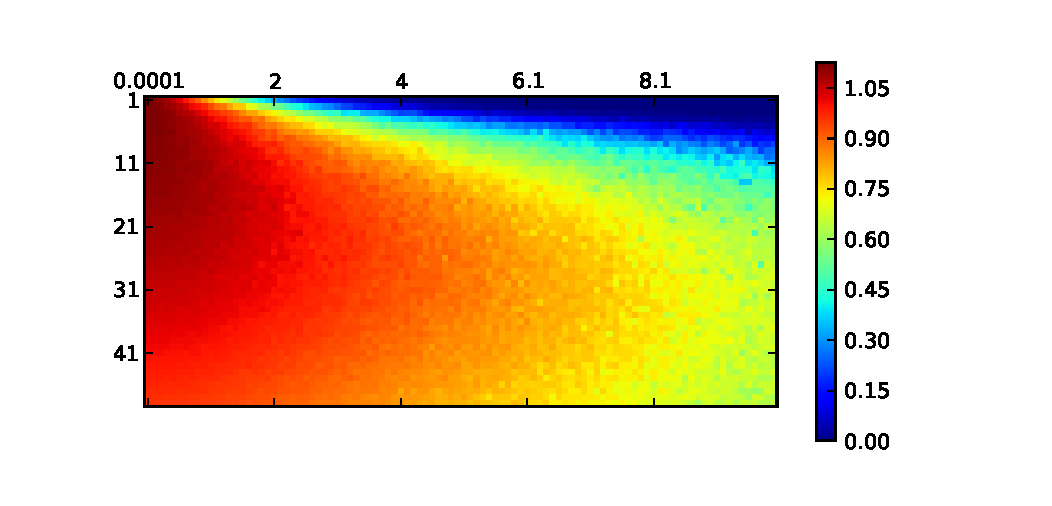
\includegraphics{fit}
\caption{This is a plot of $D/D_0$ as calculated using the fitting method. $1$ (red) is good. \bf{ In all of the matshow plots, the y-axis is $b$ and the x-axis is $s$}}
\end{figure} 
We see that the calculated diffusion matches the LRT estimate for $s=0$ as expected, but is smaller for larger $s$ with small $b$.
This might mean that this "measurement" might be the correct one.

\section{Resistor network}
Before I proceed with to ERH, I wanted to make sure the other measurement we have would produce meaningfull results.
\begin{figure}[H]
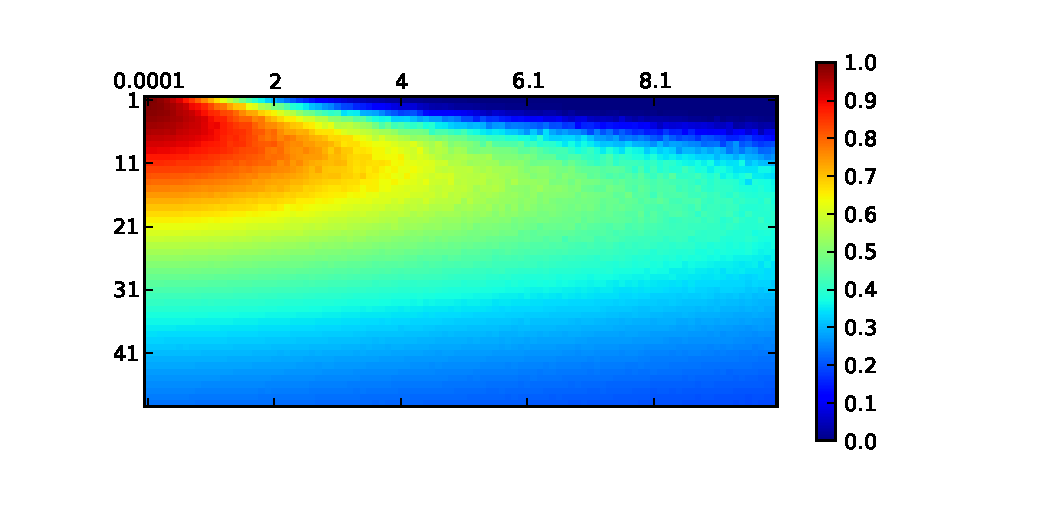
\includegraphics{new_resnet}
\caption{This is a plot of $D/D_0$ as calculated using the "new" resistor network method.}
\end{figure} 
We can see that the resistor network fails even for $s=0$. I am not sure whether to attribute it to the method (meaning SLRT doesn't hold for $b=40$ and $s=0$, or to 
a mistaken implementation.

To debug, I have returned to the basics. Using a $1000x1000$ matrix, with $b=40$ and $s=0$, I have pseudo - inverted the $W$ matrix to obtain $W^{-1}$. 
Then, I constructed a zero-filled vector $I$, with $(-1)$ on site 250, and $(+1)$ on site 750 (there are 1000 sites overall).
\begin{figure}[H]
\includegraphics{voltage_b40}
\caption{This is a plot of $V=W^{-1}I$}
\end{figure} 
We can see in the plot large voltage bumps where the current has been applied. We can also see a voltage drop after $b$ sites. I have tried to take the voltage bump out of the calculation, by measuring the voltage after the voltage drop. The resulting $D(s,b)$ is plotted next:
\begin{figure}[H]
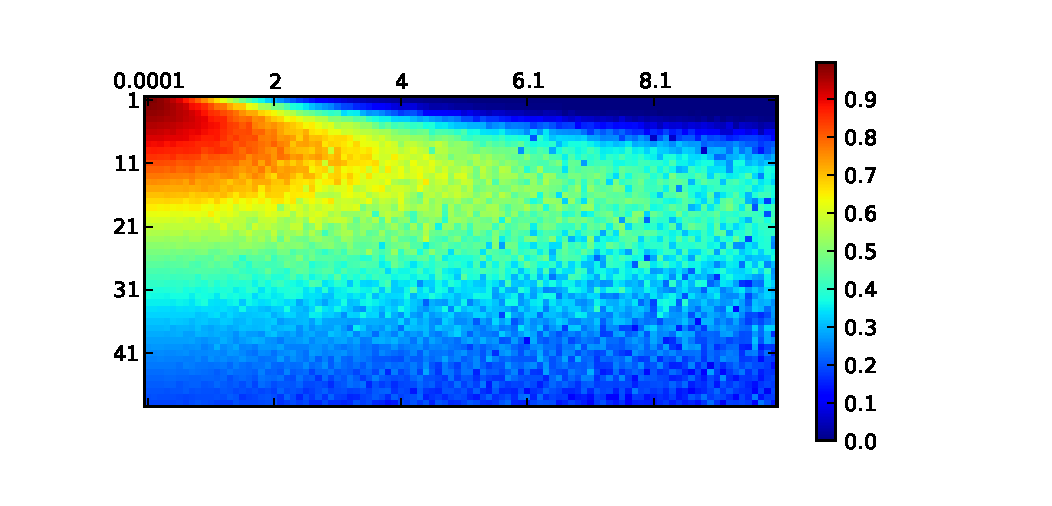
\includegraphics{resnet3}
\caption{This is a plot of $D/D_0$, using the resistor network method, measuring voltage $b$ steps inwards.}
\end{figure} 
As we can see this mearly decreased $D$ by a small amount. This image is less streamlined because it is not averaged like the "new resistor network" is.

\section{ERH}
So of the two measurements, resistor network and eigenvalue fitting, only eigenvalue fitting holds for large $b$, so we will use this from now on.

To apply the ERH method, we first have to find the cut-off $w*$, or, as is easier, find $\epsilon*$.
\begin{align}
\iint_{w>w*} \rho(r,\epsilon) dr d\epsilon = P_c \\
\iint_{\epsilon<\epsilon*} b\cdot f(\epsilon) d\epsilon = b\cdot\frac{\epsilon*}{2\sigma} = P_c\\
\epsilon* = \frac{2\sigma P_c}{b}
\end{align}

Now, we integrate over $min(w(r,\epsilon*),w(r,epsilon))r^2$ to obtain:
\begin{align}
   D_\textrm{ERH} &= \frac{b(b+1)(2b+1)}{6}(\int_0^{\epsilon*}w_0e^{-\epsilon*}\frac{d\epsilon}{2\sigma} +  \int_{\epsilon*}^{2\sigma} w_0e^{-\epsilon})\frac{d\epsilon}{2\sigma} \\
   &= \frac{b(b+1)(2b+1)}{6} w_0\left(e^{-\epsilon*}\epsilon*+e^{-\epsilon*}-e^{-2\sigma}\right)\frac{1}{2\sigma}\\
   &=\frac{b(b+1)(2b+1)}{6} w_0 \left( e^{-2\sigma\frac{P_c}{b}}\left(2\sigma\frac{P_c}{b} + 1\right) - e^{-2\sigma}\right)
\end{align}

The correction is indeed in the correct area, as can be seen here:
\begin{figure}[H]
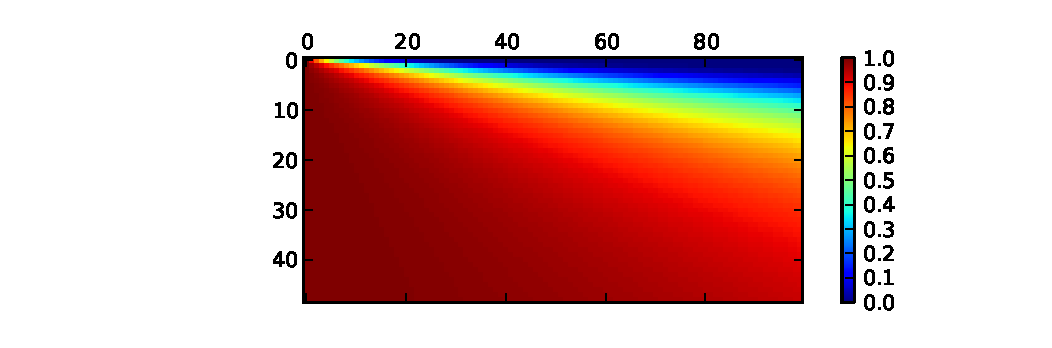
\includegraphics{BANDED_ERH}
\caption{This is a plot of $D_\textrm{ERH}/D_0$, with $P_c=1$}
\end{figure}

But I could not yet find a perfect fit for $P_c$. As an example I plot here $D/D_0$ for $b=21$, together with some options for $P_c$, but none match good enough:
\begin{figure}[H]
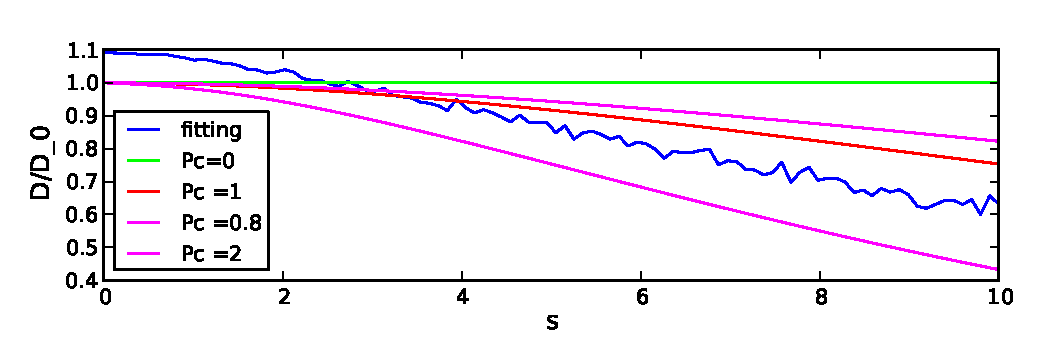
\includegraphics{b21}
\caption{This is a plot of $D/D_0$, using the fitting method, together with $D_\textrm{ERH}$ for several options of $P_c$.}
\end{figure}
\end{document}
